% Sesi 1: perintah dasar dan koordinat.
\documentclass{article}
\usepackage{tikz}
\usepackage[margin=2cm]{geometry}
\begin{document}
\begin{figure}[ht]
\centering
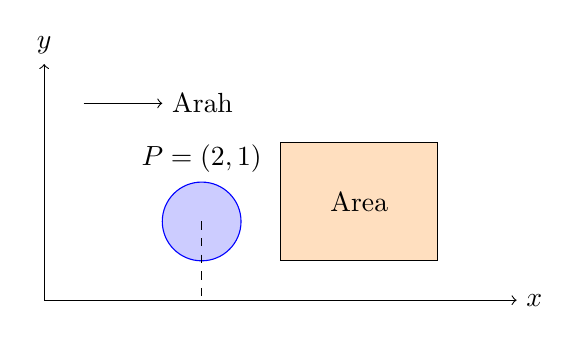
\begin{tikzpicture}
  \draw[->] (0,0) -- (6,0) node[right] {$x$};
  \draw[->] (0,0) -- (0,3) node[above] {$y$};
  \filldraw[fill=blue!20,draw=blue] (2,1) circle (5mm);
  \node[above] at (2,1.5) {$P=(2,1)$};
  \fill[orange!25] (3,0.5) rectangle (5,2);
  \draw (3,0.5) rectangle (5,2);
  \node at (4,1.25) {Area};
  \draw[dashed] (2,1) -- (2,0);
  \draw[->] (0.5,2.5) -- +(1,0) node[right] {Arah};
\end{tikzpicture}
\caption{Ilustrasi koordinat, bentuk, warna, dan label.}
\end{figure}
\end{document}
